%%%%%%%%%%%%%%%%%%%%%%%%%%%%%%%%%%%%%%%%%%%%%%%%%%%%%%%%%%%%%%%%%%%%%%%%%%%%%%%%%
%% LaTeX documentation for the implementation of the initialization routines for
%% synchronous generator in DTR Sheets.
%%
%% (c) 2022 RTE
%% Developed by Grupo AIA
%%
%%%%%%%%%%%%%%%%%%%%%%%%%%%%%%%%%%%%%%%%%%%%%%%%%%%%%%%%%%%%%%%%%%%%%%%%%%%%%%%%%
\documentclass[a4paper,11pt]{article}
\usepackage[utf8]{inputenc}
\usepackage[tmargin=2cm, bmargin=2cm, lmargin=3cm, rmargin=3cm]{geometry}
\usepackage{hyperref}
\usepackage{amsmath}
\usepackage{graphicx}
\usepackage{caption}
%\captionsetup[figure]{font=footnotesize,labelfont=footnotesize,margin=2cm}
\captionsetup[figure]{font=scriptsize,labelfont=scriptsize,margin=2cm}
\usepackage{xcolor}
\usepackage[cbgreek]{textgreek} % for the Dynawo "omega" font
\usepackage{biblatex}
\addbibresource{initialization.bib}
\usepackage{appendix}



%%%%%%%%%%%%%%%%%%%%%%%%%%%%%%%%%%%%%%%%%
%% From here on, our short-hand macros:
%%%%%%%%%%%%%%%%%%%%%%%%%%%%%%%%%%%%%%%%%
\newcommand{\code}[1]{\texttt{#1}}  % for code snippets
\newcommand{\Dynawo}{Dyna\textomega o} % but it doesn't show in bold

%% Our colors (for backgrounds and code listings):
\definecolor{light-gray}{gray}{0.9}
\definecolor{dark-gray}{gray}{0.4}
\definecolor{light-blue}{RGB}{64,64,255}
\definecolor{dark-blue}{RGB}{16,16,64}
\definecolor{dark-green}{RGB}{16,128,16}

%% More sensible colors for hyperref links:
\hypersetup{
  colorlinks = true, % color links instead of ugly boxes
  urlcolor   = blue, % color of external hyperlinks
  linkcolor  = dark-blue, % color of internal links
  citecolor  = red   % color of citations
}

%% Math macros
\renewcommand{\Re}{\ensuremath{\operatorname{Re}}}
\renewcommand{\Im}{\ensuremath{\operatorname{Im}}}
\providecommand{\abs}[1]{\lvert#1\rvert}
\newcommand{\Vpdr}{\ensuremath{V_{\textrm{PDR}}}}
\newcommand{\Ipdr}{\ensuremath{I_{\textrm{PDR}}}}
\newcommand{\Spdr}{\ensuremath{S_{\textrm{PDR}}}}
\newcommand{\Ytr}{\ensuremath{Y^{\textrm{(tr)}}}}
\newcommand{\Ysh}{\ensuremath{Y^{\textrm{(sh)}}}}
\newcommand{\Sgen}{\ensuremath{S_{\textrm{gen}}}}
\newcommand{\Pgen}{\ensuremath{P_{\textrm{gen}}}}
\newcommand{\Qgen}{\ensuremath{Q_{\textrm{gen}}}}
\newcommand{\Saux}{\ensuremath{S_{\textrm{aux}}}}
\newcommand{\Paux}{\ensuremath{P_{\textrm{aux}}}}
\newcommand{\Qaux}{\ensuremath{Q_{\textrm{aux}}}}



%%%%%%%%%%%%%%%%%%%%%%%%%%%%%%%%%%%%%%%%%
%% The document starts here
%%%%%%%%%%%%%%%%%%%%%%%%%%%%%%%%%%%%%%%%%

\title{\Dynawo{} Model-Validation Tool: initialization routines for synchronous
  generators in DTR Sheets}

\author{Grupo AIA}
\date{
  \today
} 



\begin{document}
\maketitle
\tableofcontents

\begin{abstract}
  This document describes in detail the routines within the \Dynawo{} Model-Validation
  tool that calculate the initialization values for all elements in the various DTR
  Sheets~\cite{DTRhome}.
\end{abstract}





\section{Overview}

Although the producer is expected to supply his own model for the generator, he cannot
be asked to also provide the correct initialization values for all the the case
scenarios prescribed by the DTR Sheets. Such initialization is dependent on many other
parameters that vary from sheet to sheet, such as the connection reactances, the values
of P, Q, or V at the connection point (PDR bus), etc.  Therefore the \Dynawo{}
Model-Validation tool performs its own internal calculations to find out the correct
initialization values for the generator, auxiliary load, etc.; on a case-by-case basis.

For the moment being, \emph{the approach consists in assuming that the
topology on the producer's side is restricted to a small set of
variants}, which enables us to calculate the quantities analytically
by means of relatively simple load-flow (LF) formulas. In the future
we do not rule out some other approach providing greater freedom, such
as running the cases through one or more passes in
\emph{DynaFlow}~\cite{Dynawo} until a valid steady state is achieved.


\section{Allowed topology variants}

For our analytic LF approach to work, the topology on the producer's side \emph{must} be
one of these eight variants:
\begin{description}
\item[S:] single gen/WT/PV unit
\item [S+i:] single gen/WT/PV unit + Line (represents an ``internal network'')
\item [S+Aux:] single gen/WT/PV unit + Aux Load 
\item [S+Aux+i:] single gen/WT/PV + Aux Load + Line
\item [M:] multiple WT/PV units
\item [M+i:] multiple WT/PV units + Line
\item [M+Aux:] multiple WT/PV units + Aux Load
\item [M+Aux+i:] multiple WT/PV units + Aux Load + Line
\end{description}

\noindent\textbf{Note for Zone-1 tests:} for the isolated tests of individual WT/PV
units without plant-level control (i.e., the so-called ``Zone 1'' tests), the only
allowed topology is \textbf{``S''}.

As we can observe, there are here two main groups: single-unit vs.\ multiple-unit
topologies. Then in each case one may model, if desired, an ``internal network'' via a
single \code{Line} object, and auxiliary loads via a single \code{Load} object.  These
topologies are depicted in Figs.~\ref{fig:topoS}--\ref{fig:topoM}. If the producer's
topology deviates from these assumptions, our analytic LF calculations will result in
incorrect initialization parameters for the generators and therefore the simulations may
start at an unstable state.

\begin{figure}[ht]
  \centering
  \hfill
  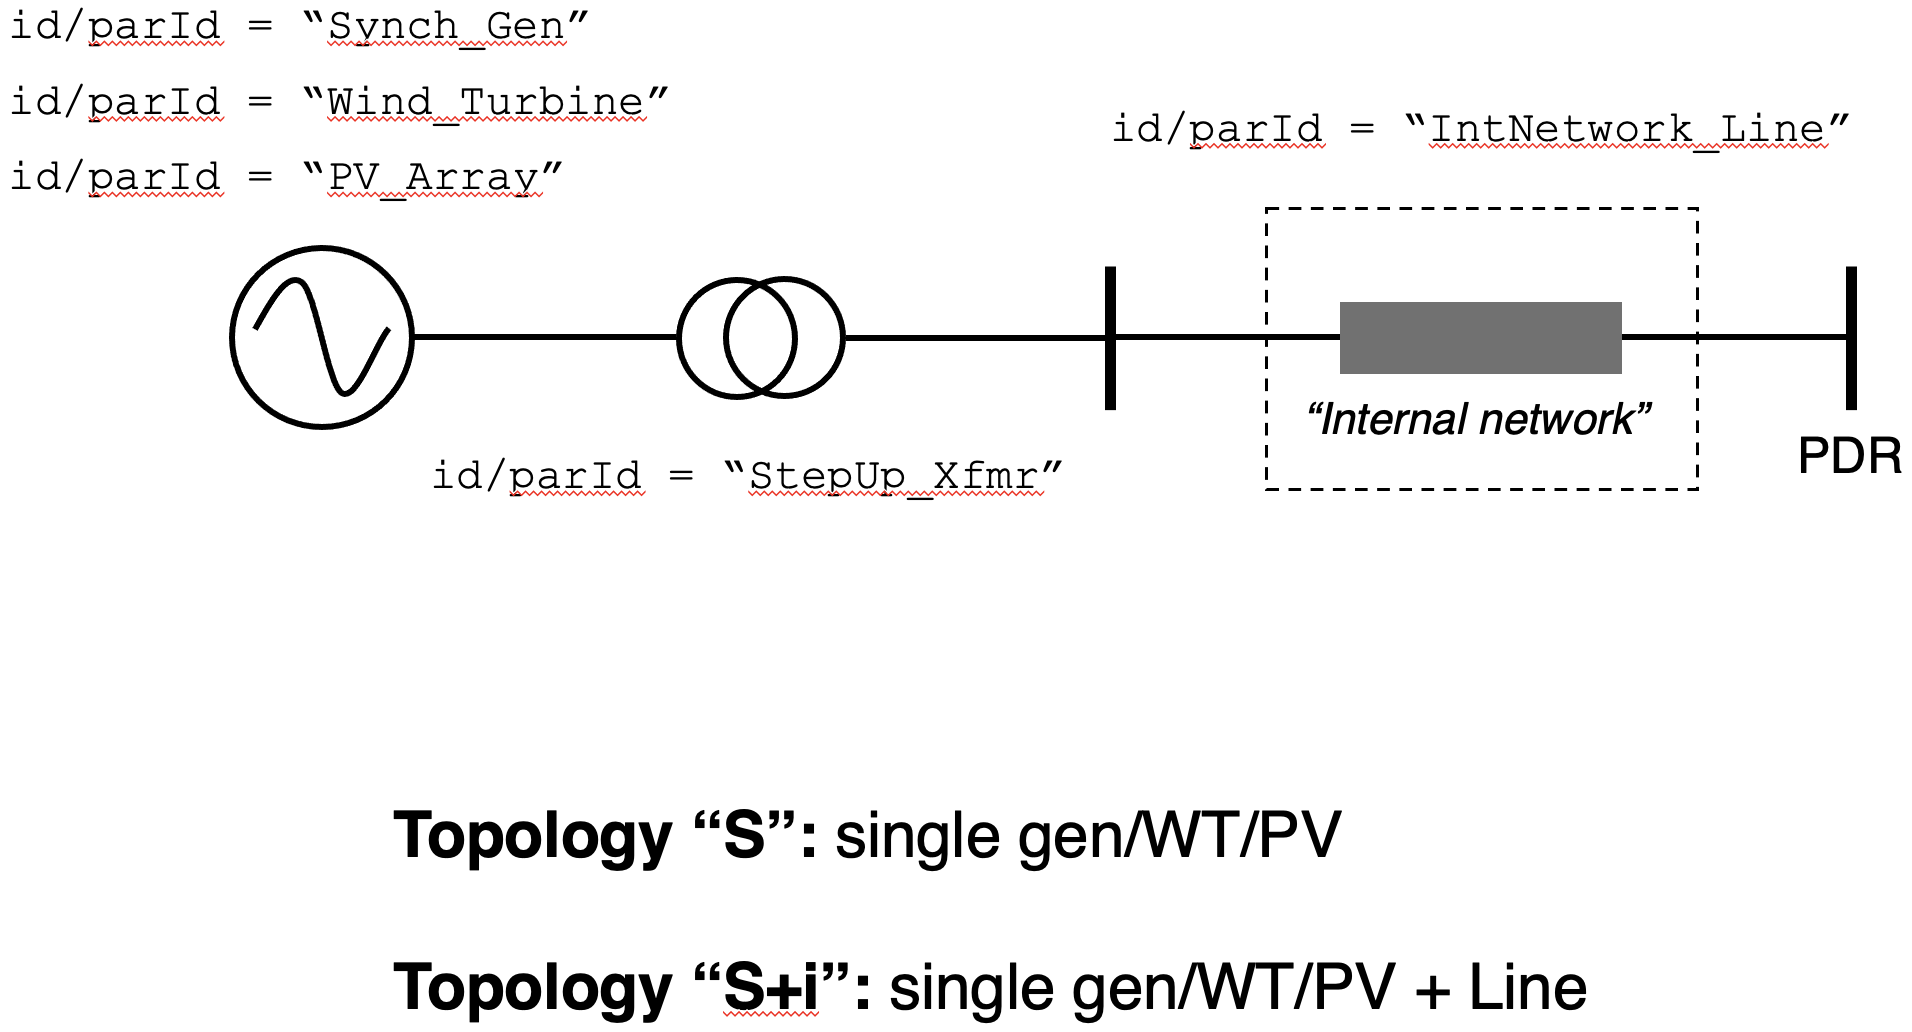
\includegraphics[width=0.45\textwidth]{topology_S.png}
  \hfill
  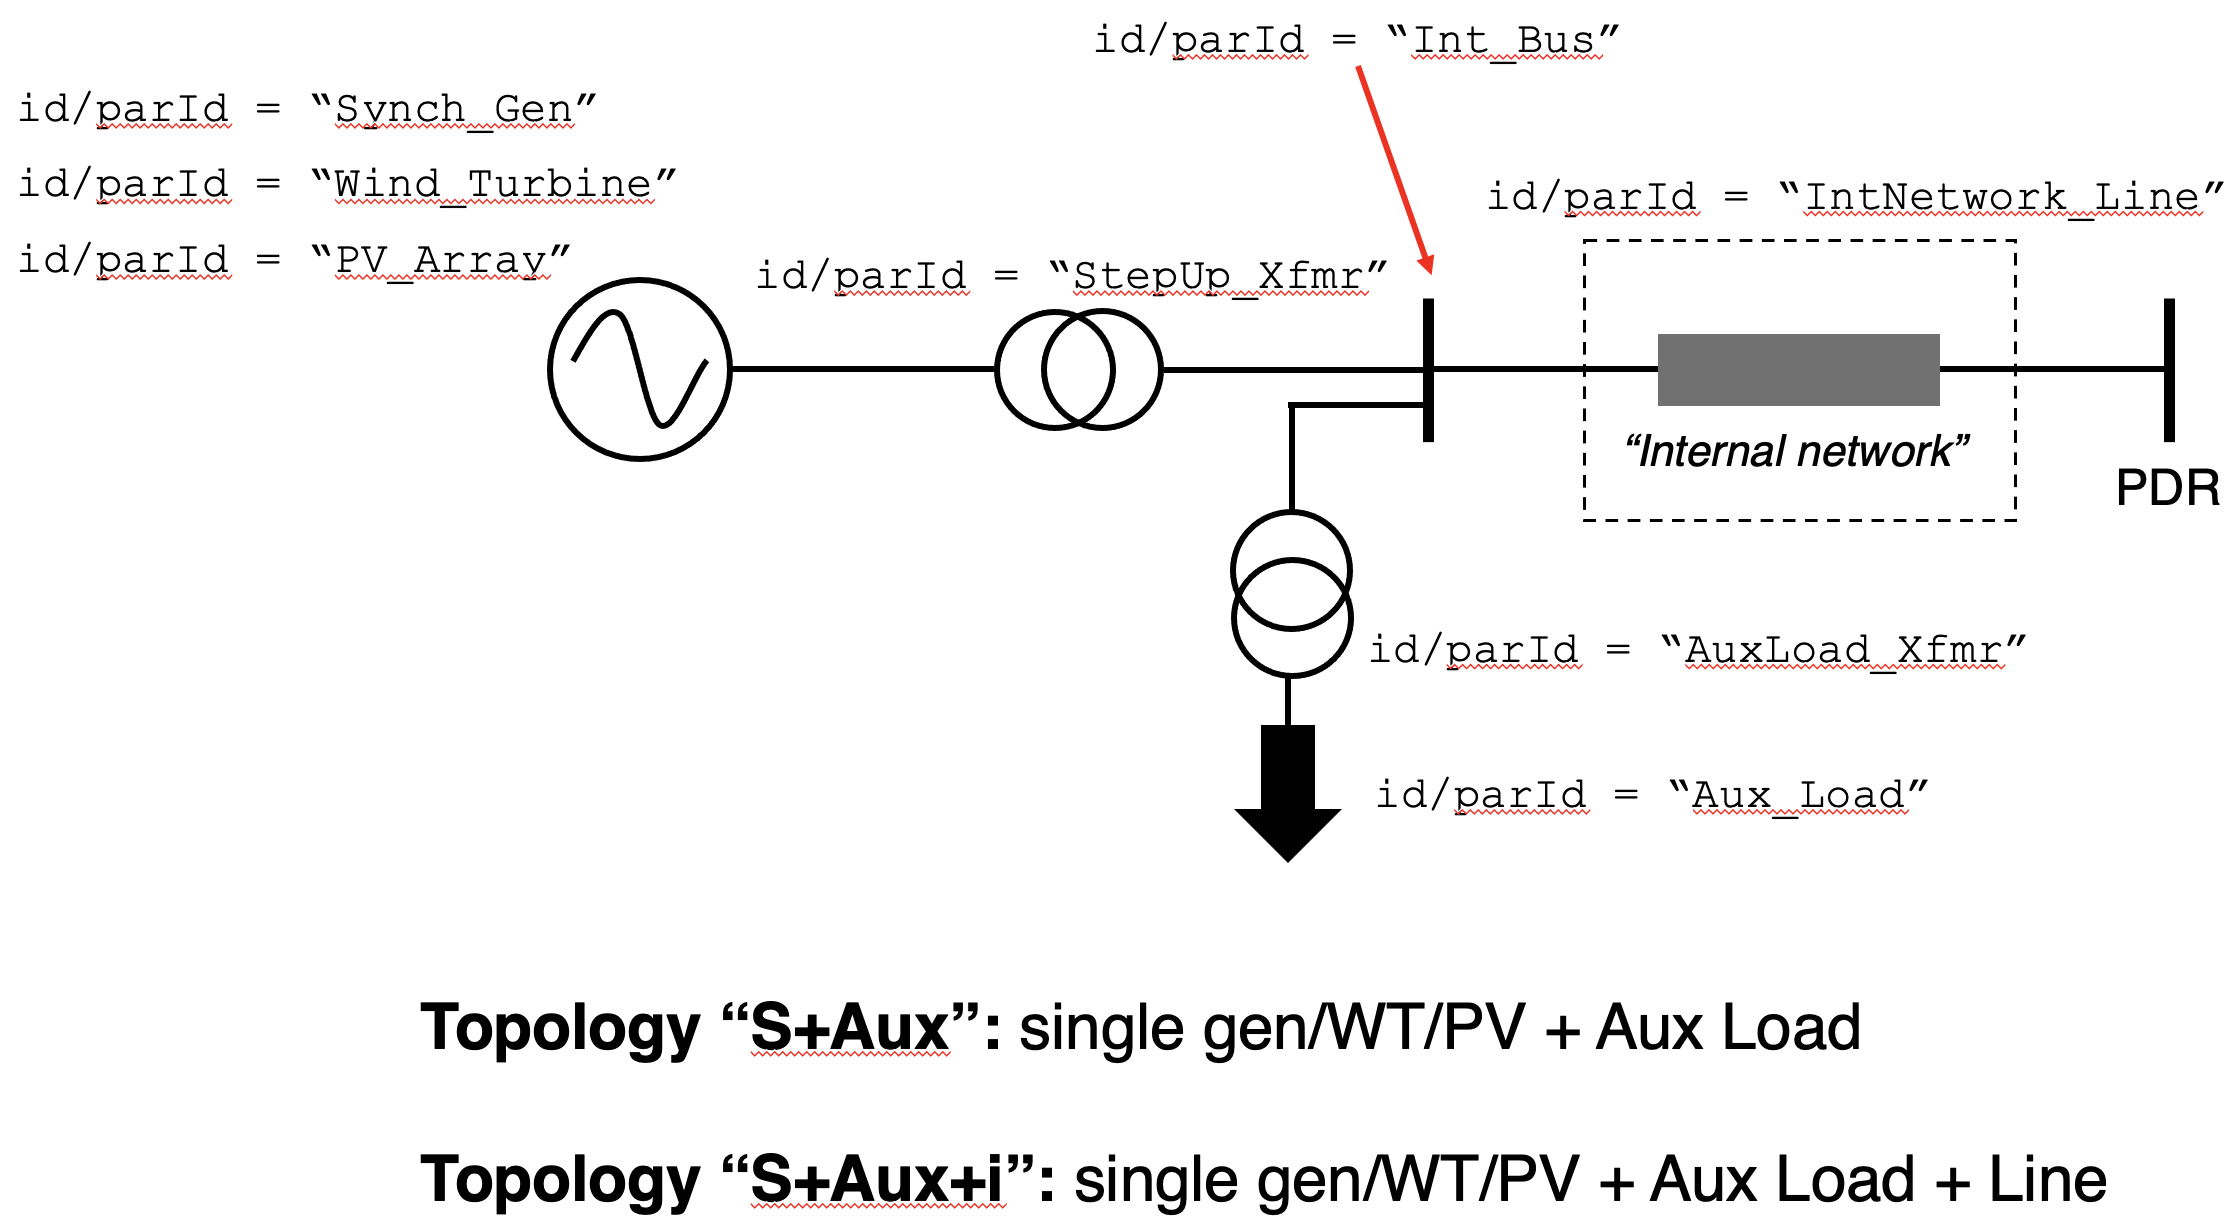
\includegraphics[width=0.45\textwidth]{topology_S_AuxLoad.png}
  \hfill
  \caption{Allowed topologies for cases with a single unit.}
  \label{fig:topoS} 
\end{figure}

\begin{figure}[ht]
  \centering
  \hfill
  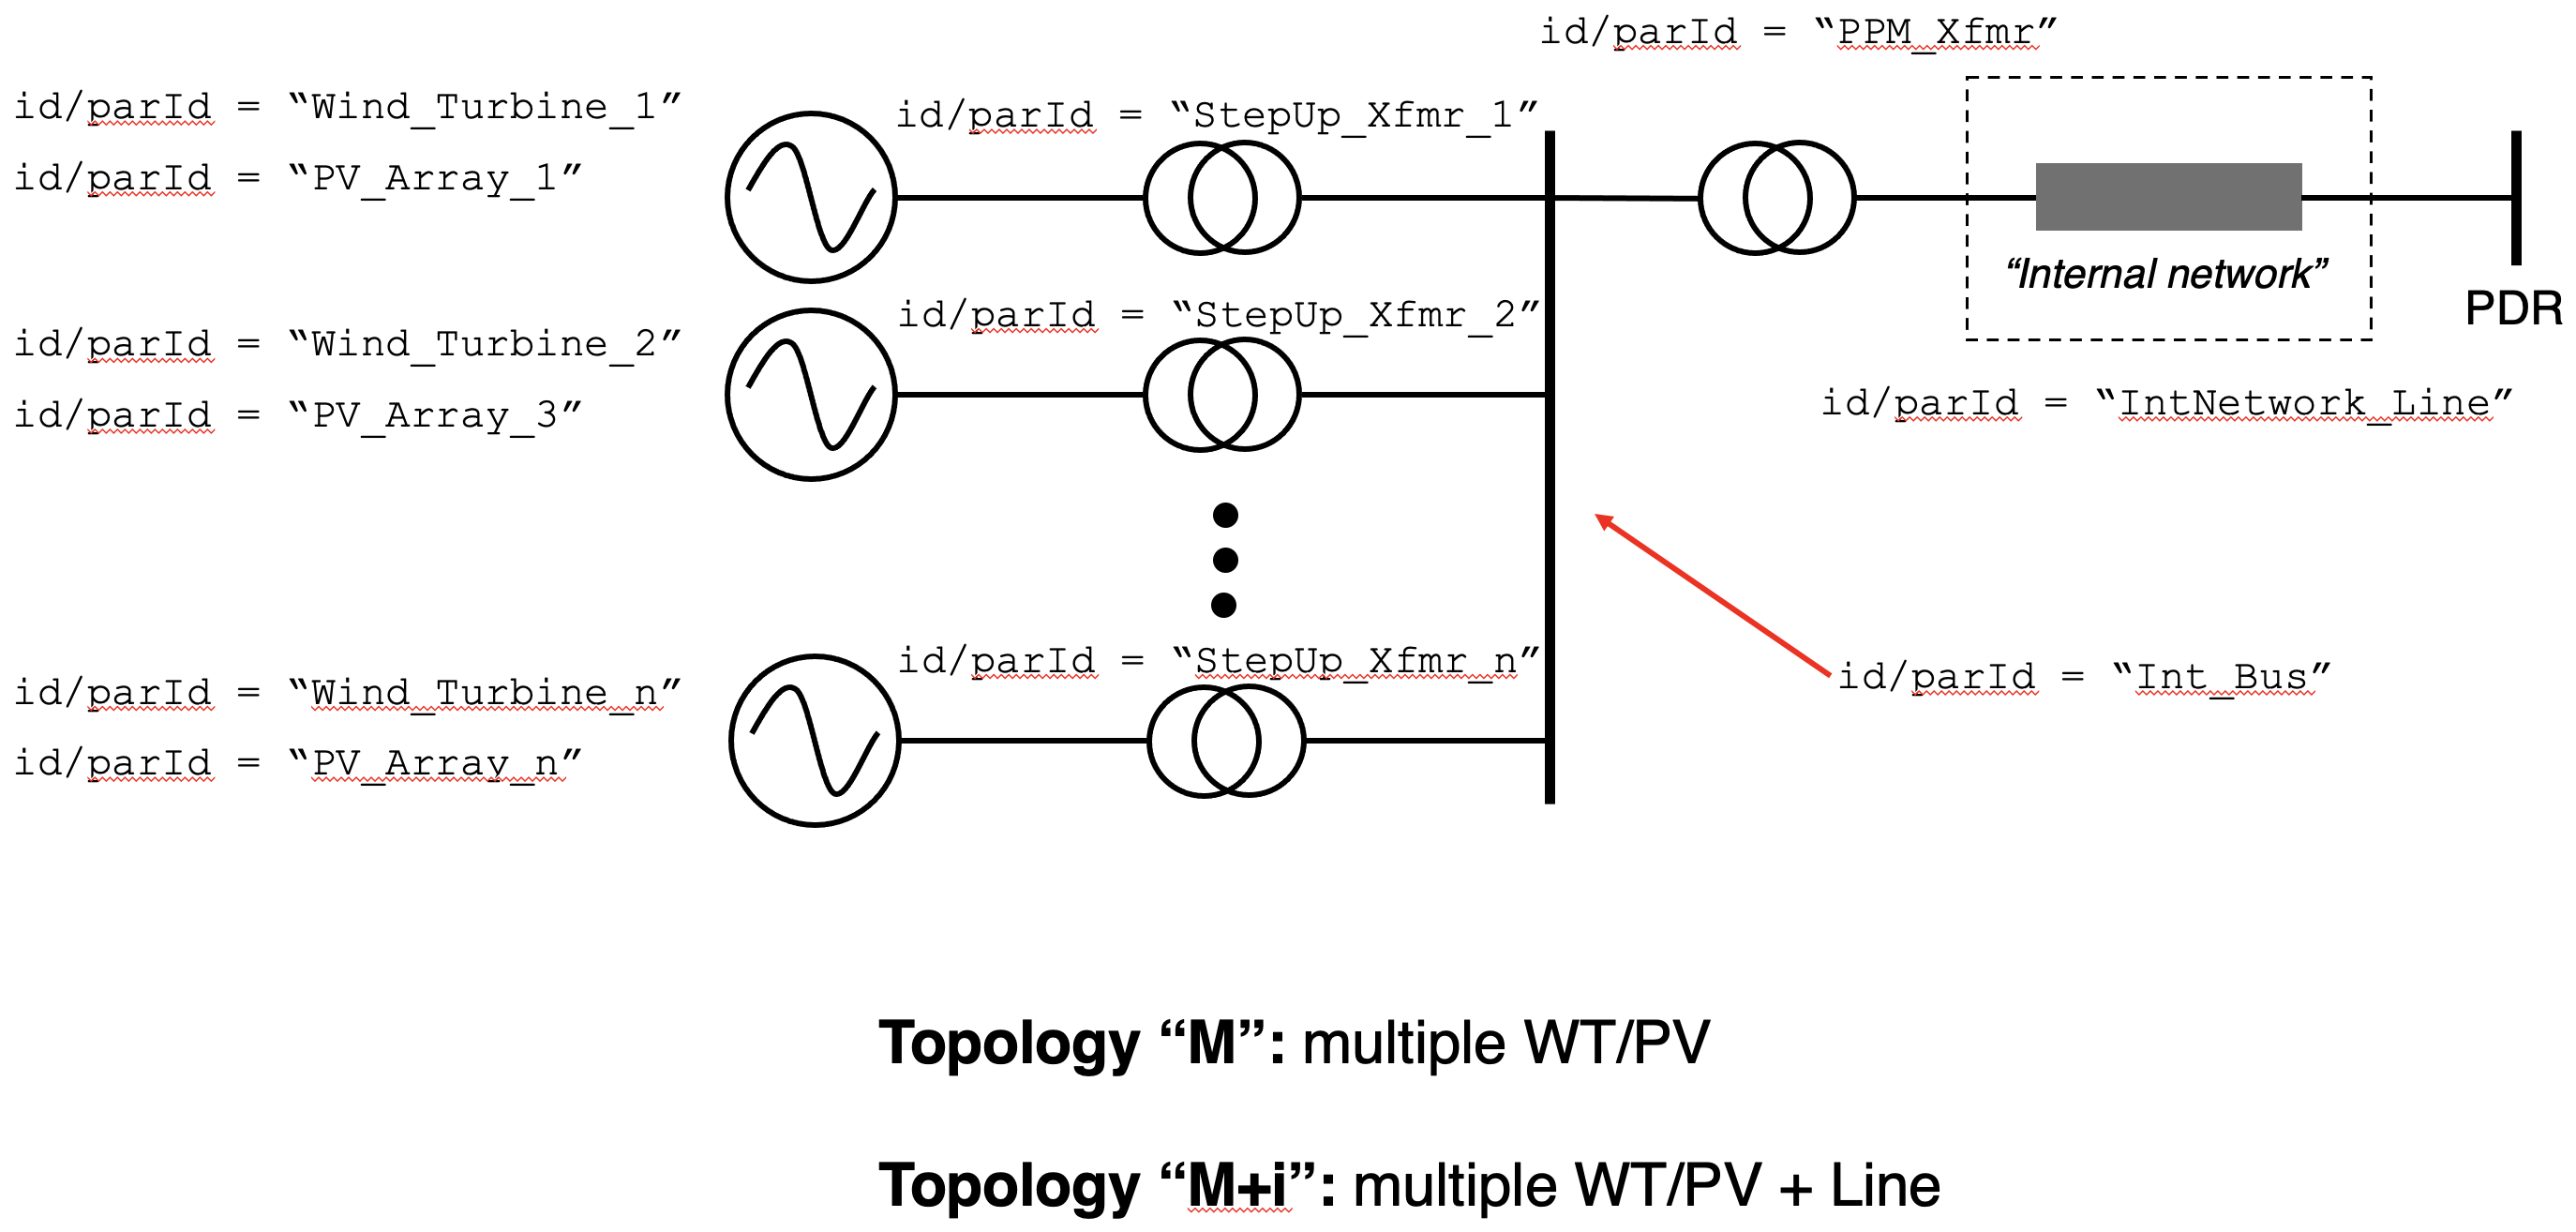
\includegraphics[width=0.45\textwidth]{topology_M.png}
  \hfill
  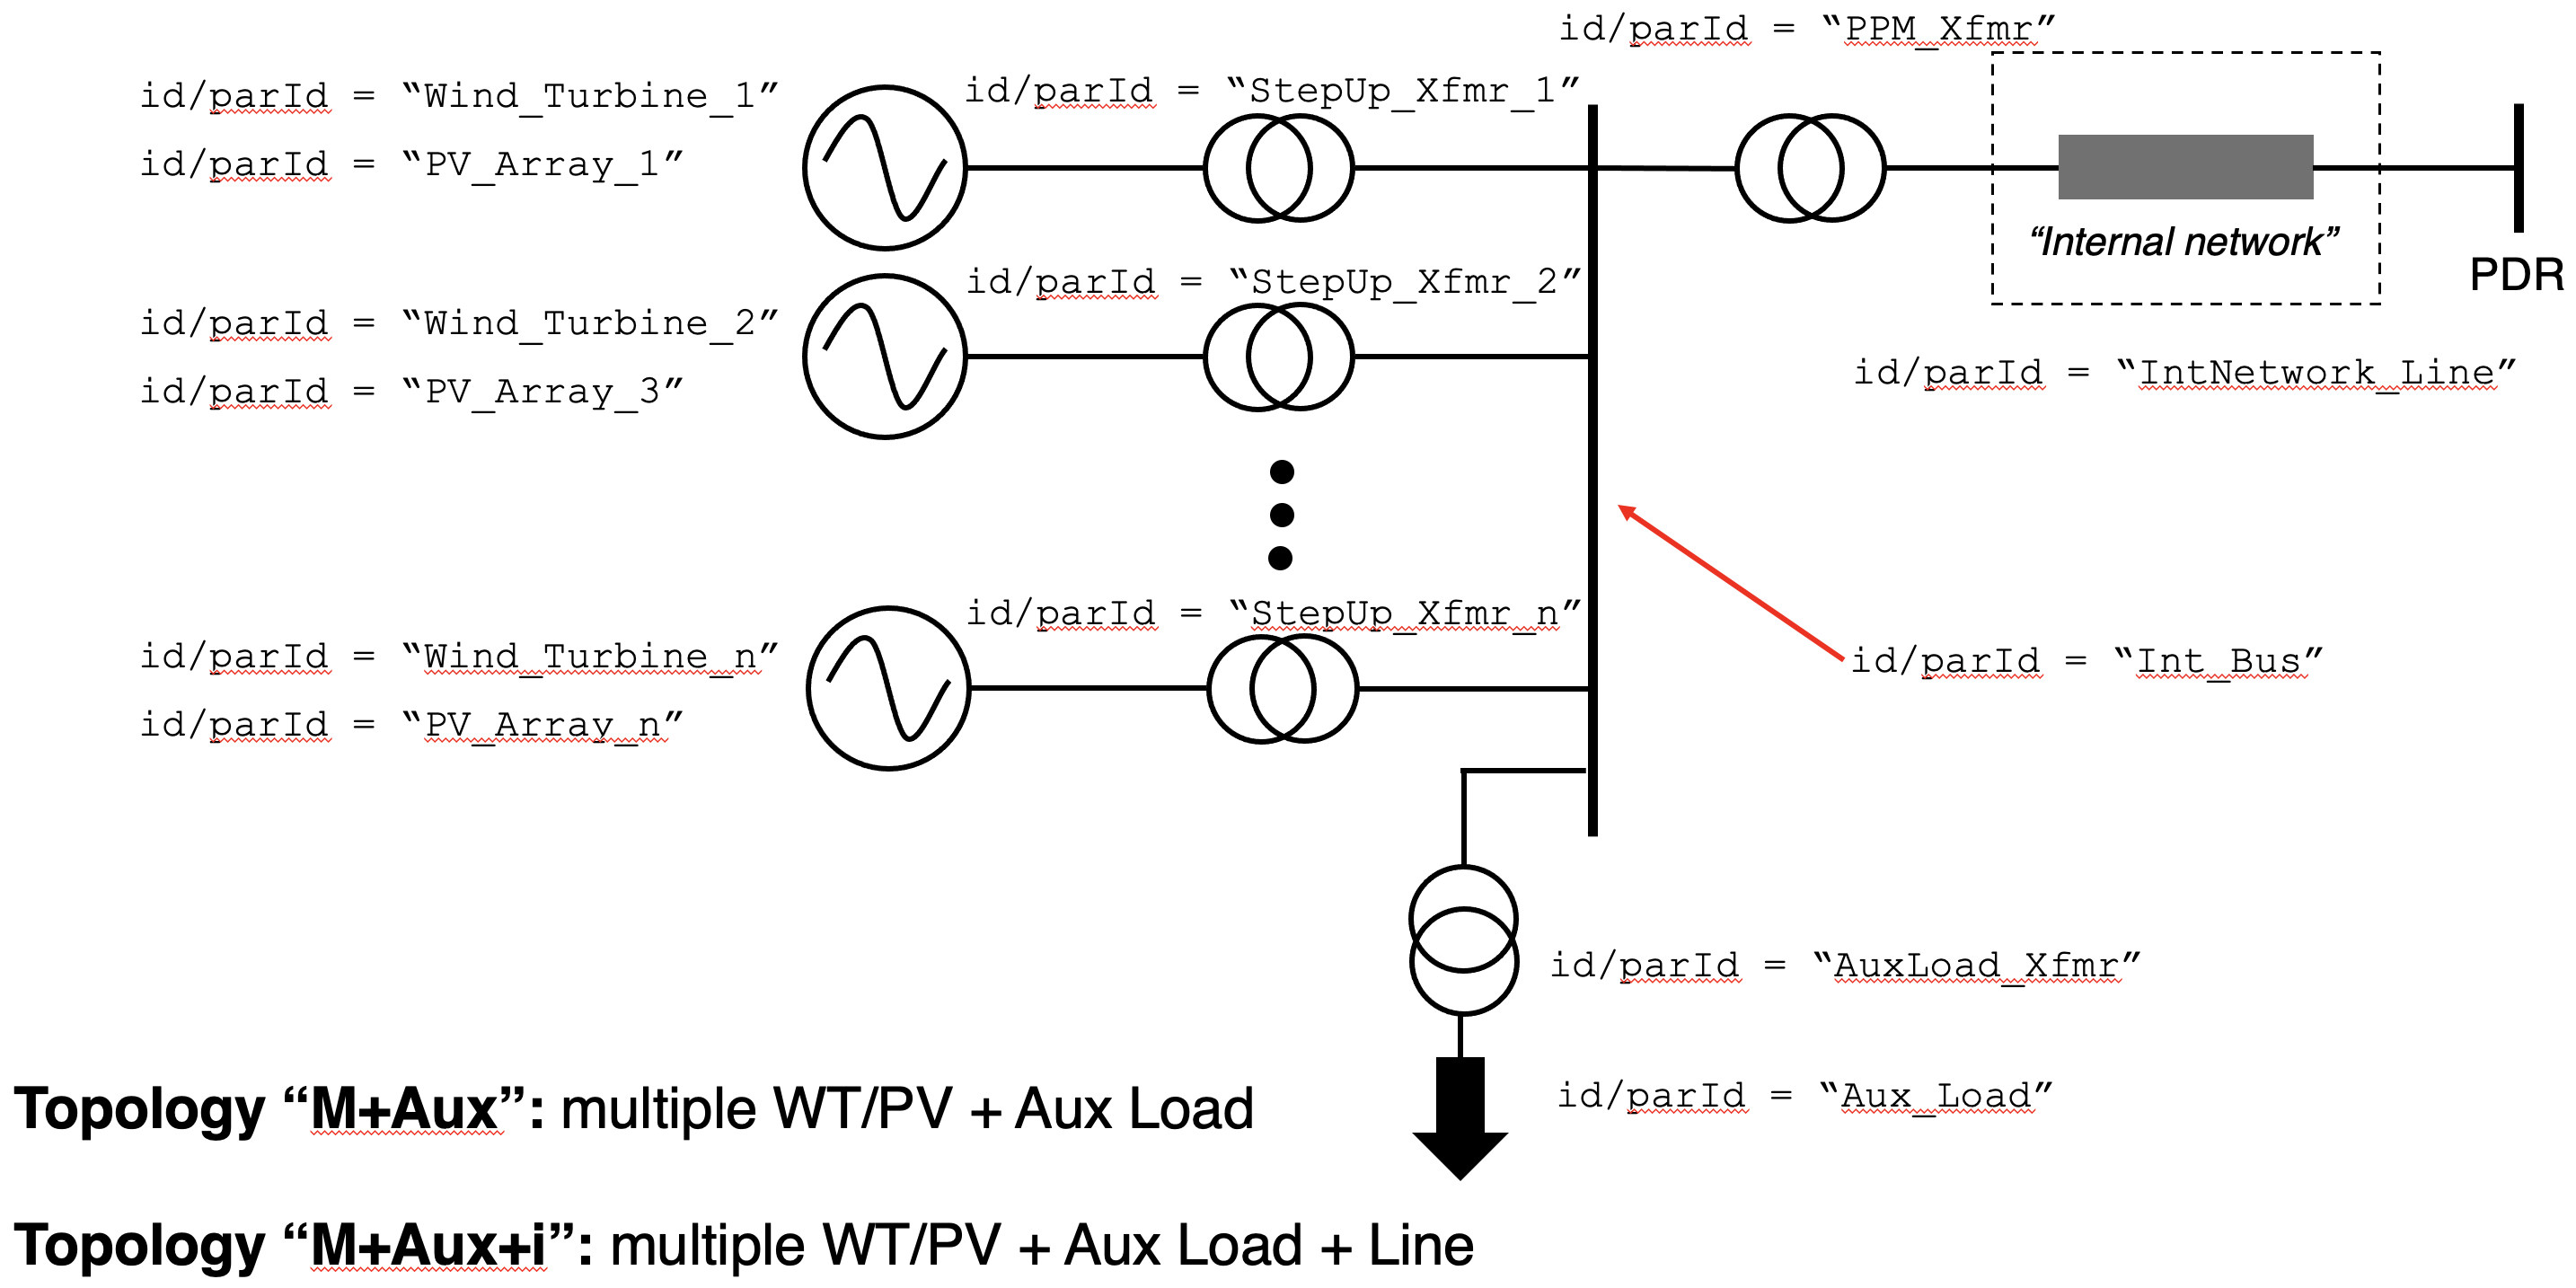
\includegraphics[width=0.45\textwidth]{topology_M_AuxLoad.png}
  \hfill
  \caption{Allowed topologies for cases with multiple units.}
  \label{fig:topoM} 
\end{figure}




\section{Strategy for the calculation}
Looking at the above topologies, and knowing that:
\begin{itemize}
\item the topology on RTE's side always contains an Infinite Bus (except Fiche I10, in
  which there are only loads)
\item the magnitudes V, P, Q are always prescribed at the PDR bus
\end{itemize}
It is easy to see that a general strategy for calculation is as follows:
\begin{enumerate}
\item First choose the angle reference (zero) to be at the PDR. Therefore all complex
  magnitudes V, I, S are known at the PDR bus.
\item Start by calculating the complex voltage at the Infinite Bus. This is the only
  initialization value we will need on RTE's side. In addition, we may keep the value of
  the angle in order to perform a global shift at the end, in case we wanted the
  Infinite Bus to be the angle reference instead (although this is not really
  necessary).
\item We then proceed from the PDR bus towards the other side, section by section. The
  calculation will vary depending on the topology:
  \begin{itemize}
  \item If there is only a line or a transformer followed by a generator unit, the
    calculation simply involves the formulas of a pi-model equivalent.
  \item If there is an auxiliary load, the calculation will involve a second-order
    algebraic equation (a standard two-bus load-flow), since this load specifies
    a constant PQ value.
  \item If there are multiple generating units, the calculation needs one additional
    input from the user: the sharing fractions of their respective PQ injections (we
    obtain this from the initialization values given by the user in his
    \code{Producer.par} file).
  \end{itemize}
\end{enumerate}




\section{LF calculations for Topologies S and S+i}

We start by noticing that the DTR Sheets specify three quantities at the point of
connection, the PDR bus: voltage modulus and the complex flow $S=P+jQ$. This allows one
to easily propagate the complex voltage and complex currents on either side of the PDR
bus, \emph{independently}. Actually, these LFs do not involve any quadratic equation at
all, as it will be shown now (this will be different in the next sections, when a PQ
auxiliary load is present).

The plan proceeds as follows, in outline mode:
\begin{itemize}
\item First LF: calculate the complex voltage at the RTE bus, needed to initialize the
  Infinite Bus model. We may use this voltage angle to perform a global phase shift, so
  that this bus becomes the reference (i.e., angle zero).
\item Second LF (case S+i): calculate the complex voltage and current at the other end
  of the line representing the producer's ``internal network'', if it is modeled.
\item Third LF: calculate the complex voltage and current on the low-voltage side of the
  generator transformer, thus obtaining the generator PQ output as well.
\end{itemize}



\subsection{First LF: RTE's side}
Let us focus first on the problem to the right of the PDR bus in Fig.~\ref{fig:topoS},
that is, RTE's network side. We start with this side first because, once $V_\infty$ is
solved for, we can shift phase globally so that $V_\infty$ sets the reference (zero
angle).  This is not strictly necessary, but it is more convenient for analysts when
they look at the results. Having in mind the pi-model equivalent of the connection
line(s) and using current conservation plus the fundamental power equation $S=VI^*$, one
has:
\begin{equation*}
  \Ipdr = \frac{\Spdr^*}{\Vpdr^*} - \Vpdr \Ysh_1
        = ( \Vpdr - V_\infty ) \Ytr
\end{equation*}

Since we will be repeating the same sort of calculation to the left of the PDR
bus, it is useful to make this calculation more general by rewriting it in terms
of a pi-model equivalent circuit as shown in Fig.~\ref{fig:pimodel_LF}:
\begin{equation*}
  I_{1\rightarrow 2} = \frac{S_1^*}{V_1^*} - V_1 \Ysh_1
                     = ( V_1 - V_2 ) \Ytr
\end{equation*}
Rearranging this equation,
\begin{equation*}
  \frac{S_1^*}{V_1^* \Ytr} - V_1 \frac{\Ysh_1}{\Ytr}
  = V_1 - V_2 \,, 
\end{equation*}
we easily obtain the complex voltage at terminal 2:
\begin{equation}
  V_2 = V_1 \left(1 + \frac{\Ysh_1}{\Ytr} \right) - \frac{S_1^*}{V_1^* \Ytr}
  \label{eq:complex_V}
\end{equation}

If instead of an infinite bus we had modeled a real generator on RTE's side (as is the
case of Fiche I8), we would also need to calculate the PQ injection of the
generator. For that, we calculate the corresponding current $I_2$. Using again the sign
conventions indicated by the arrows in Fig.~\ref{fig:pimodel_LF}, this current is:
\begin{equation}
  I_2 = ( V_1 - V_2 ) \Ytr - V_2 \Ysh_2 \,
  \label{eq:complex_I}
\end{equation}
so that the total complex injection at the bus is:
\begin{equation}
  S_2 \equiv P_2 + j Q_2 = V_2 I_2^*
  \label{eq:complex_S}
\end{equation}
And finally the initialization values of P and Q for such generator are straightforward
to obtain, simply by subtracting from $S_2$ the value (with the proper sign) of the
equivalent PQ loads, if any are present (see Fiche I8).


\begin{figure}
  \centering
  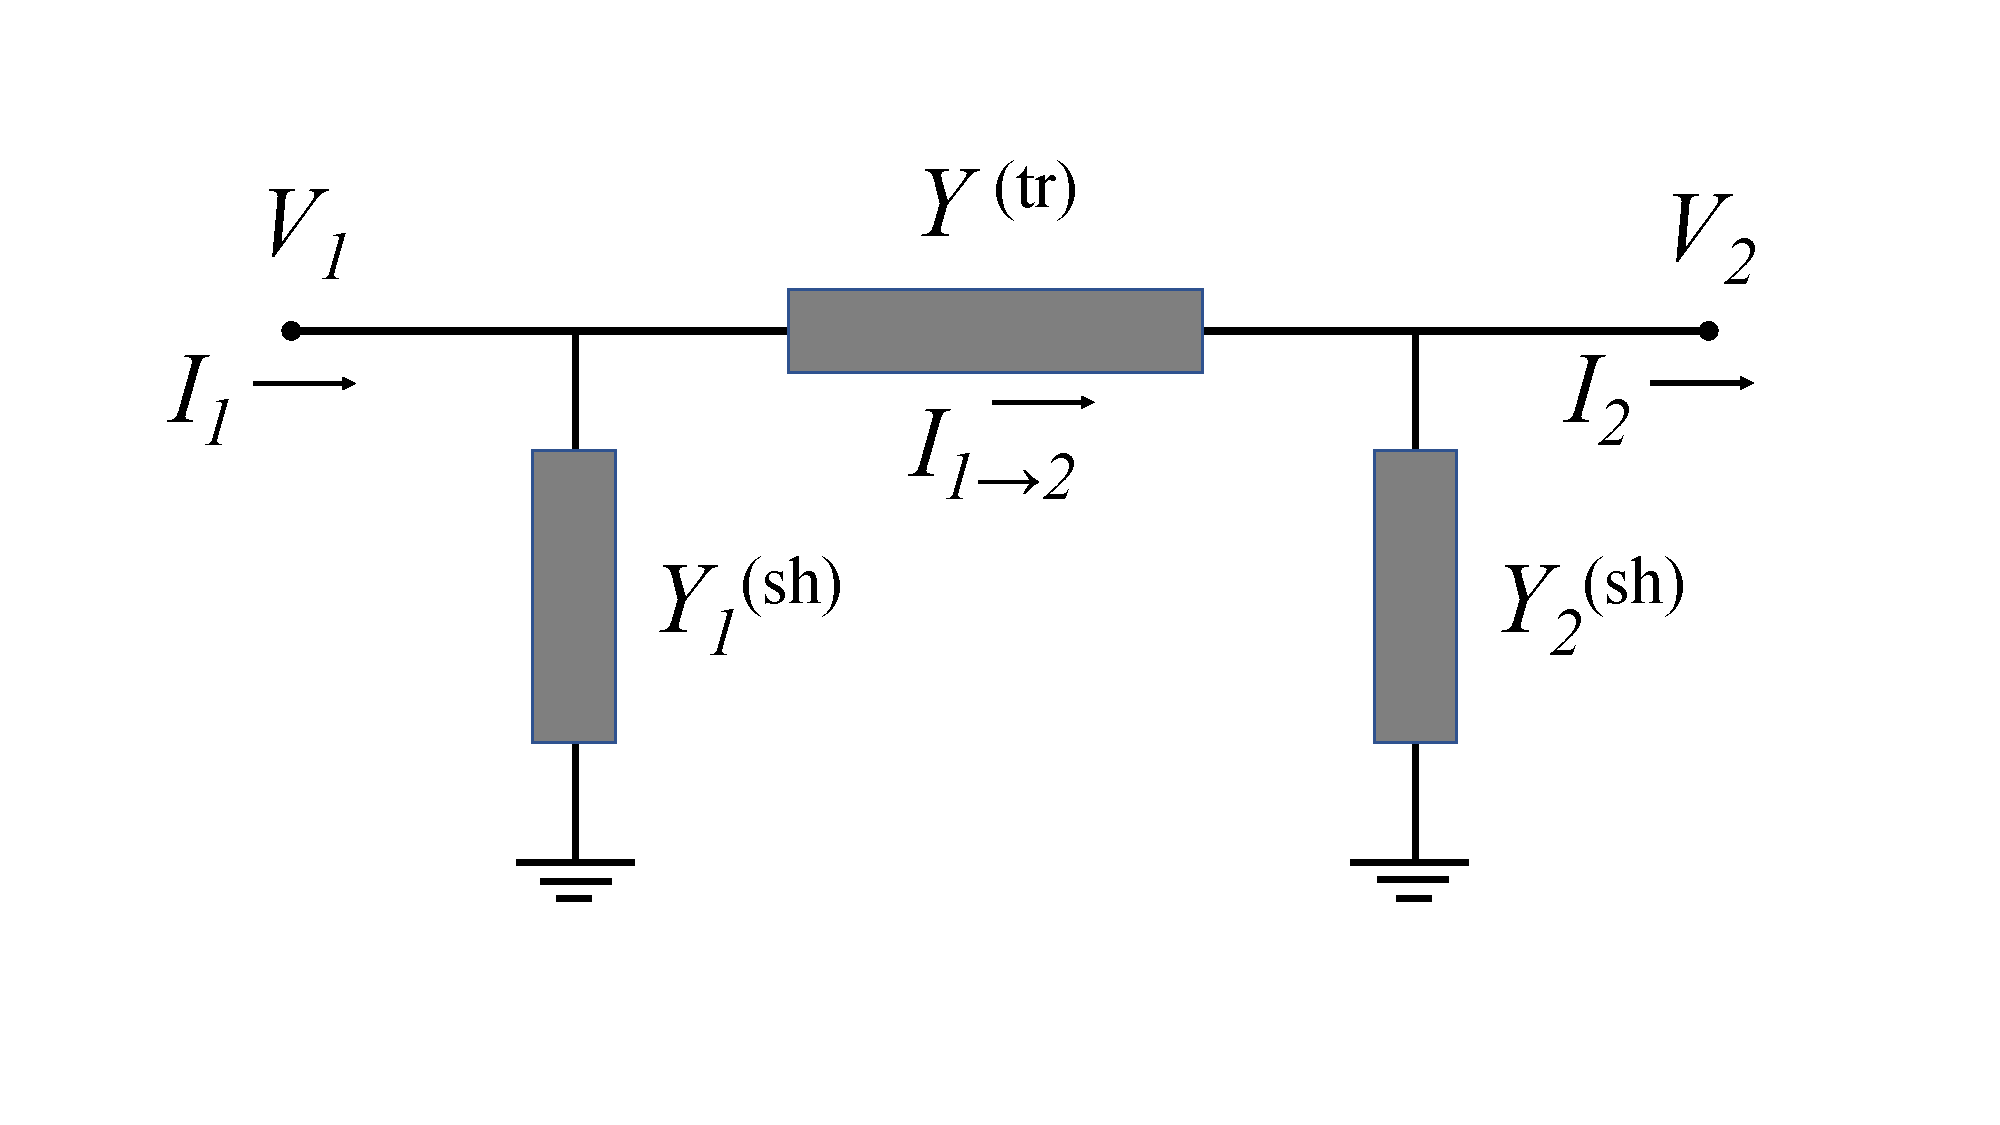
\includegraphics[width=0.6\textwidth]{pi_model_circuit}
  \caption{This is the pi-model circuit involved in the basic ``loadflow'' that we solve
    at several steps of the procedure. In our calculations, Terminal 1 always represents
    the bus where both complex voltage and complex current (or, equivalently, complex
    voltage and P \& Q) are known. The complex voltage and current on terminal 2 are
    calculated through simple algebra (so this is not really a loadflow problem,
    strictly speaking). Notation: (tr) stands for \emph{transmission} branch; (sh)
    stands for \emph{shunt} admittance.}
  \label{fig:pimodel_LF}
\end{figure}



\subsection{Second LF: the producer's ``internal network'' (case S+i)}

If the producer has modeled an internal network (by means of a Line object), we will
need to propagate the complex voltage and current to the other side, the internal bus.

The calculation is exactly the same as in the previous subsection, using again
expressions~\eqref{eq:complex_V} and \eqref{eq:complex_I}.  We will keep the convention
that terminal 1 is the one at which magnitudes are known (in this case, the PDR bus),
and terminal 2 is where we need to calculate voltages, currents, and so on.  The signs
of the resulting currents and power flows will be correct if we are consistent with the
arrows: in this particular case here, it means that the values of inputs $P_1 + j Q_1$
need to have their signs flipped, compared to the values used in the previous
subsection.  To be sure, $P_1$ is positive in the previous subsection and it is negative
here, as per the \Dynawo{} convention (which is, ``loads are positive'').

Therefore we will be using a common function \code{calc\_pimodel\_pf()}, but we
will have to be careful when handling the signs of its inputs and outputs.


\subsection{Third LF: the generating unit}

As it can be seen in the diagram for topologies S and S+i in Fig.~\ref{fig:topoS}, it
now suffices to calculate the voltage and current at the low-voltage side of the
generator's step-up transformer.

Again, the calculation is is exactly the same as in the previous two subsections.  This
time terminal 1 is the HV side of the step-up transformer (which is the the PDR bus in
case of topology S, and the internal bus in case of topology S+i).  Therefore we will be
calling again the common function \code{calc\_pimodel\_pf()}, being careful when
handling the signs of inputs and outputs. One thus obtains the complex voltage with
expression~\eqref{eq:complex_V} and the PQ output of the generator through
expressions~\eqref{eq:complex_I} and \eqref{eq:complex_S}.




\section{LF calculations for Topologies S+Aux, S+Aux+i}

The calculations for these topologies are very similar to the previous ones.  The only
difference lies in the third LF, since the presence of an auxiliary load forces us to
calculate a proper two-bus load-flow problem, i.e. solve a quadratic equation (for which
it is straightforward to get the solution algebraically, in closed form).

The plan proceeds as follows, in outline mode:
\begin{itemize}
\item First LF: same as in the case of topologies S and S+i.
\item Second LF (case S+Aux+i): same as in the case of topology S+i.
\item Third LF: calculate voltage and current on the low-voltage side of the
  \emph{auxiliary load} transformer first. We need to know this current in order
  to calculate the next and final step.
\item Fourth LF: calculate voltage and current on the low-voltage side of the
  \emph{generator} transformer, thus obtaining the generator PQ output as well.
\end{itemize}


\subsection{Third LF: the auxiliary load circuit}

As it can be seen in Fig.~\ref{fig:topoS} (right hand side), the generator output PQ
cannot be calculated until we know how much current is going into the auxiliary load
circuit vs.\ the generator circuit.

Since the PQ consumption of the load is specified, and the complex voltage at the HV
side of the load transformer is known, one can calculate the voltage at the load and
thus the current.  This is a standard two-bus power flow problem, which involves solving
a quadratic equation.

Let us solve it in closed form. The circuit is again a simple pi-model model
representing the auxiliary load transformer.  As in the rest of this paper, we adopt the
convention that terminal 1 represents the bus where both voltage and current are
known--although in this particular case, the current is unknown!  Terminal 2 is where
the auxiliary load is connected to. Therefore equation we need to solve is:
\begin{equation*}
  (V_1 - V_2) \Ytr = \frac{S_2^*}{V_2^*} + \Ysh_2 V_2 \;,
\end{equation*}
where $V_1$ is known, $S_2$ is known (the load's PQ), and $V_2$ should be solved for. We
will solve this in terms of the real and imaginary parts of $V_2$. To prepare for that,
let us rearrange this equation:
\begin{equation*}
  (\Ytr + \Ysh_2) V_2 - \Ytr V_1  +  \frac{S_2^*}{V_2^*}  = 0
\end{equation*}
and now divide the equation by suitable constants:
\begin{equation*}
  \left( \frac{\Ytr + \Ysh_2}{\Ytr} \right) \frac{V_2}{V_1} - 1
  + \left( \frac{S_2^*}{\Ytr \abs{V_1}^2} \right) \frac{V_1^*}{V_2^*}  = 0
\end{equation*}
so that we can redefine the variable and the constants as follows:
\begin{equation}
  \label{eq:V2defs}
  \begin{split}
  v & \equiv \left( \frac{\Ytr + \Ysh_2}{\Ytr} \right) \frac{V_2}{V_1} \\
  \sigma & \equiv \frac{\left( \Ytr+\Ysh_2 \right)^* S_2^*}{\abs{\Ytr}^2 \, \abs{V_1}^2}
  \end{split}
\end{equation}
in order to simplify the equation:
\begin{equation}
  v - 1 + \frac{\sigma}{v^*}  = 0
\end{equation}

It is now easy to solve this equation in the complex variable $v$ by using the
real and imaginary parts, $v_x + j v_y$. Let us first multiply by $v^*$:
\begin{equation*}
  \abs{v}^2 - v^* + \sigma = 0 \;.
\end{equation*}
The two equations are then:
\begin{align*}
  v_x^2 + v_y^2 - v_x + \sigma_x  & = 0 \\
  v_y + \sigma_y  & = 0
\end{align*}
From this we readily obtain $v_y = -\sigma_y$, and therefore arrive at this
quadratic equation for $v_x$:
\begin{equation*}
  v_x^2 - v_x + \sigma_x  + \sigma_y^2 = 0
\end{equation*}
For which the solution is:
\begin{equation*}
  v_x = \frac{1}{2} \pm \sqrt{\frac{1}{4} - \sigma_x - \sigma_y^2}
\end{equation*}
Here the correct solution branch is obviously the one with the plus sign, as this would
yield a high voltage ($v=1$) if the loads were zero ($\sigma=0$), as expected. Therefore
the complex voltage is:
\begin{equation}
  v = \frac{1}{2} + \sqrt{\frac{1}{4} - \sigma_x - \sigma_y^2} - j \sigma_y
\end{equation}
from which one readily obtains $V_2$ by undoing the definitions in
Eq.~\eqref{eq:V2defs}.

Lastly, the net current that flows from terminal 1 into the auxiliary loads
circuit can be calculated as:
\begin{equation}
  I_{\text{aux}} = (V_1 - V_2) \Ytr + V_1 \Ysh_1
\end{equation}
This quantity will be needed in the next section.



\subsection{Fourth LF: the generator circuit}

Here the calculation is very similar to the third LF in the case of topologies S and
S+i, except that we first need to subtract from $I_1$ the current $I_{\text{aux}}$ that
is drawn by the auxiliary loads circuit (which was calculated in the previous
subsection).  Once we do that, both voltage and current are known at terminal 1 and one
can calculate voltage and current at terminal 2 (i.e., the generator terminals, also the
LV side of the step-up transformer).

Then the PQ output of the generator is simply given by $\Sgen = S_2 = V_2
I_2^*$.




\section{LF calculations for Topologies M and M+i}

The procedure is almost the same as that of Topologies S and S+i, with one crucial
difference: when attempting to perform what we called the third LF, one needs more data;
namely, how the net injection is \emph{shared} among the several generating units. We
obtain these proportionality factors for P and Q from the user input. More precisely, we
read the existing initialization values of $P_0$ and $Q_0$ for each generator $k$ in the
\code{Producer.par} file provided by the user, and calculate the proportionality factors
in a straightforward way:
\begin{equation}
  \begin{split}
    \lambda_P^{(k)} & = \frac{P_0^{(k)}}{\sum_{i=1}^n P_0^{(i)}} \\
    \lambda_Q^{(k)} & = \frac{Q_0^{(k)}}{\sum_{i=1}^n Q_0^{(i)}}
  \end{split}
\end{equation}
where $n$ is the number of generating units. We then simply apply these proportionality
factors to the net injection $S_1$ of equation~\eqref{eq:complex_V}, to obtain the
complex voltages and PQ values at each generator terminals, with equations
\eqref{eq:complex_V}--\eqref{eq:complex_S}.




\section{LF calculations for Topologies M+Aux and M+Aux+i}

The procedure follows the same steps as those for Topologies S+Aux and S+Aux+i, up to
the third LF (for the auxiliary load).  Then, the fourth loadflow is different: one
first needs to subtract from $I_1$ the current $I_{\text{aux}}$ that is drawn by the
auxiliary load circuit. The new net value of the injection thus becomes $S_1 = V_1 (I_1
- I_{\text{aux}})^*$, and we can then calculate the complex voltages and PQ values at
each generator terminals as in the previous section, using their corresponding
$\lambda_P^{(k)}, \lambda_Q^{(k)}$ sharing factors.




\newpage
\appendix
\appendixpage
\addappheadtotoc

\section{Pi-model equivalent parameters}

In this section we describe how to obtain the pi-model parameters $\Ytr, \Ysh_1,
\Ysh_2$ from the physical parameters that we can read from the \Dynawo{} case
files.


\subsection{Single line}

This is quite simple, as \Dynawo's Line model is already in the form of a
pi-model equivalent. Pay attention, though: the shunt admittances are already
divided by two (they follow Eurostag's convention: they are
``half-admittance'').  Therefore one has:
\begin{equation}
  \begin{split}
    \Ytr   & = \frac{1}{\code{line\_RPu} + j \, \code{line\_XPu}} \\
    \Ysh_1 & = \code{line\_GPu} + j \, \code{line\_BPu} \\
    \Ysh_2 & = \code{line\_GPu} + j \, \code{line\_BPu} 
  \end{split}
\end{equation}


\subsection{Multiple parallel lines}

In this case one would simply \emph{add} the admittances, as both the transmission and
the shunt admittances are connected in parallel to each other, respectively.
\begin{equation}
  \begin{split}
    \Ytr   & = \sum_{i=1}^n \frac{1}{\code{line\_RPu}_i + j \, \code{line\_XPu}}_i \\
    \Ysh_1 & = \sum_{i=1}^n \code{line\_GPu}_i + j \, \code{line\_BPu}_i \\
    \Ysh_2 & = \sum_{i=1}^n \code{line\_GPu}_i + j \, \code{line\_BPu}_i 
  \end{split}
\end{equation}





\subsection{Transformers}

For transformers, one needs to pay attention to the internal modeling used in \Dynawo.
This is the equivalent circuit and conventions:
\begin{quote}
  \begin{verbatim}
               I1  r                I2
    U1,P1,Q1 -->---oo----R+jX-------<-- U2,P2,Q2
  (terminal1)                   |      (terminal2)
                               G+jB
    r=U2/U1                     |
                               ---
  \end{verbatim}
\end{quote}
In the following, we will use the notation $Z \equiv R+jX$ (transmission branch)
and $Y_m \equiv G + jB$ (magnetizing branch).  We will use this now this circuit
to obtain the values of its pi-model equivalent $\Ytr, \Ysh_1, \Ysh_2$ in terms of
$Z$ and $Y_m$. Note that, for this calculation, we will be using the convention
that current $I2$ flows in the other direction (see Fig.~\ref{fig:pimodel_LF}),
but this does not affect the final formulas.

Let us first recall the pi-model circuit in Fig.~\ref{fig:pimodel_LF}. It is
straightforward to write the circuit equations:
\begin{equation*}
  \begin{split}
    I_1 & = (V_1 - V_2) \Ytr + V_1 \Ysh_1 \\
    I_2 & = \left(V_1 - V_2\right) \Ytr - V_2 \Ysh_2
  \end{split}
\end{equation*}
We will re-arrange it in this form, which reminds us better of the familiar
matrix equation $I = Y V$:
\begin{equation}
  \label{eq:pimodelIV}
  \begin{split}
    I_1 & = \left( \Ytr + \Ysh_1 \right) V_1 - \Ytr V_2 \\
    I_2 & = \Ytr V_1 - \left( \Ytr + \Ysh_2 \right) V_2
  \end{split}
\end{equation}
Now the aim is to obtain the analogous set of equations for the transformer's
equivalent circuit, so that we can then identify each of these four
coefficients between the two.

The transformer circuit can be solved from first principles as follows. We will
use the following notation:
\begin{itemize}
\item $e_1, i_1$: voltage and current at the ideal section of the transformer,
  on terminal 1 side.
\item $e_2, i_2$: voltage and current at the ideal section of the transformer,
  on terminal 2 side.
\end{itemize}
Looking at the diagram, we readily observe that $e_1=V_1$ and $i_1=I_1$. Now the
two fundamental relations of the transformer are the following:
\begin{align*}
    r & \equiv \frac{e_2}{e_1}  &  & \text{definition of the tap ratio} \\
    e_1 i_1^* & = e_2 i_2^* &  & \text{energy conservation (ideal transformer)} \\
\end{align*}

For $I_1$, we obtain, step by step:
\begin{equation*}
  \begin{split}
    I_1 & = i_1 \\
    & = \frac{e_2^*}{e_1^*} i_2 \\
    & = r i_2 \\
    & = \frac{r}{Z} (e_2 - V_2) \\
    & = \frac{r}{Z} (r e_1 - V_2) \\
    & = \frac{r^2}{Z} V_1 - \frac{r}{Z} V_2 \\
  \end{split}
\end{equation*}
And for $I_2$:
\begin{equation*}
  \begin{split}
    I_2 & = i_2 - V_2 Y_m \\
    & = \frac{1}{Z} (e_2 - V_2) - V_2 Y_m \\
    & = \frac{1}{Z} (r V_1 - V_2) - V_2 Y_m \\
    & = \frac{r}{Z} V_1  - \left( \frac{1}{Z} + Y_m \right) V_2
  \end{split}
\end{equation*}
Equating now the coefficients in these two last equations to those of
Eq.\eqref{eq:pimodelIV}, one finally obtains:
\begin{equation}
  \begin{split}
    \Ytr & = \frac{r}{Z} \\
    \Ysh_1 & = \frac{r(r-1)}{Z} \\
    \Ysh_2 & = \frac{1-r}{Z} + Y_m
  \end{split}
\end{equation}






%%\newpage
\clearpage
\printbibliography


\end{document}

